
%(BEGIN_QUESTION)
% Copyright 2011, Tony R. Kuphaldt, released under the Creative Commons Attribution License (v 1.0)
% This means you may do almost anything with this work of mine, so long as you give me proper credit

A technician is asked to build a recording system to continuously monitor the position of a control valve's stem.  Her solution is to couple a rugged potentiometer to the valve stem and then build a voltage divider circuit using this potentiometer to create a variable voltage representing valve stem position.  This voltage will then be read by a trend recorder and graphed over time:

$$\includegraphics[width=15.5cm]{i02212x01.eps}$$

The potentiometer is arranged to work as a rheostat (variable resistor): 0 ohms when the valve is shut and 1000 ohms when the valve is fully open, resistance linearly tracking stem motion.  What she needs now is a formula providing valve stem position (in percent, 0 to 100) from the voltage received by the recorder.  This formula will be programmed into the recorder so that the recorder may calculate and display the percentage of valve opening based on a measurement of voltage.

Write the formula below as a function of $V$ (voltage), and also calculate the voltage received by the recorder at 50\% (half-open) valve position.

\vskip 20pt

Valve position (\%) = 

\vskip 20pt

Voltage @ 50\% = \underbar{\hskip 50pt} volts

\underbar{file i02212}
%(END_QUESTION)





%(BEGIN_ANSWER)

I recommend half-credit for the formula and half-credit for the voltage at 50\%:

\vskip 10pt

Valve position (\%) = ${220 V} \over (24 - V)$

\vskip 20pt

Voltage @ 50\% = \underbar{\bf 4.44} volts

%(END_ANSWER)





%(BEGIN_NOTES)

{\bf This question is intended for exams only and not worksheets!}.

%(END_NOTES)


